% !TEX root = ../main.tex
\section{Retainer Kin} \label{kin::quies}
\DndDropCapLine{T}{hey are the last kin made by our}
\textit{creators, and as such are related to us gats, irds, and oths.
It is our duty to provide them the nourishing that our shared parents denied them.
They are, after all, our younger siblings.}

\hspace*{\fill} --- Kosmael, founder of the church of Jismuah.

After the schism, as the storm that covered the tall kin's tiding dispersed, many dark secrets were revealed.
Among these sins, the existence of the quies, or retainer kin, was of special note.
The retainer kin is a fully sentient species which, unlike the other created by the tall kin, was forced into servitude, unable to comprehend what it is to roam free or even the existence of a world outside of Jan'krug.

At some point after the tall kin secluded themselves in their mountaintop city, they decided to create this slave race to focus solely on their studies and rituals.
The quies, not understanding what freedom is, remained immersed in their tasks for centuries, continuing even after the tall ones vanished.
They continued in this meaningless loop until a gat expedition found them, still locked into servitude to their dead masters, and showed them a life unbound by chains.

\subsection*{Designed with a Purpose}
    Such as gats, irds, oths, and marsets, the quies were created by the tall kin.
    Unlike them, the quies were formed from a blend of organic and inorganic materials.
    Their bodies are made from a blend of flesh and wood, with root-like cords infused with strange fluids serving as muscles, wrapped around a framework of bone and flesh.

    Armored plates form a protective outer shell and reinforce joints.
    Quies' faces are simply a collection of holes located where sensory organs would normally be, but each has a custom made qualar mask integrated into this outer shell.
    These masks usually contain very intricate detail, and seem to be made with an almost ardent passion.

\subsection*{Functionalist at Heart}
    The quies were built to serve.
    For the first centuries of their existence, the retainer kin had a clearly defined function and were encouraged to focus purely on that role.
    While they now might have freedom, many still struggle both to find a place in the world and to relate to the creatures of it.

    The typical quies show little emotion.
    Many of them embrace a concrete purpose-such as protecting allies, completing a contract, or exploring a land --- and embrace this task as they once did.
    However, there are quies who delight in exploring their feelings, their freedom, and their relationships with others.
    The race was first welcome to Yuadrem by the church of Jismuah, and many embraced faith and mysticism, seeking higher purpose and deeper meaning.

\subsection*{Life of Subservience}
    The quies are the sentient beings that spent the most time living alongside the tall kin, and as such they are highly sought after by scholars studying them.
    While a quies can describe in great detail the daily life of a tall one, their subservient nature inhibited their curiosity.
    Not one quies is known that can recall the rituals performed by the tall kin, and most can't even tell anything about their masters other done the tasks they performed for them.

    Like the zaloths, the quies are unable to reproduce by any mean, which is probably by design.
    This, combined with the fact that their creators have almost completely disappeared from Yuadrem, makes their chances of survival as a species look very grim.
    This is countered however by the fact that, as their creators, quies don't seem to age at all.

\subsection*{New Beginnings}
    After leaving Jan'krug, the retainer kin had a very hard time adapting to the world.
    Some dedicate themselves to continuing their skill under a new patron, failing to leave behind their lives as servants.
    Others managed to learn independence, but could not abandon their craft, and became renowned artisans or merchants, being compared by many even to gat artisans.

    The quies that managed to completely break free from their bindings are regarded as special by the other members of their species, and they are met with both reverence and jealousy.
    These quies usually become adventurers, where they can blend their newfound curiosity with their armored bodies.
    Some take the plight of their kin into their hearts, and spend their lives trying to find the last remaining tall ones, aiming to learn how to create more of their own.

\subsection*{Quies Names}
    As far as is known, no tall one ever gave a name to a quies.
    Most of the retainer kin simply refer to themselves by their job, or by a name given to them by others.
    However, the quies that manage to escape their shackles and take a life of wandering are very appreciative of being given the freedom to pick their own names.
    Once chosen, a quies will guard their name with great jealousy, only sharing it with whom they trust the most.

    \paragraph{Names}
    Ba, Bal, Dreth, Eth, Feather, Fish, Gakn, Green, I, Jan, Loth, Risz, Seed, Sekru, Stand, Swim, Tis, Tlekeloo, Tlos, When, Yu, Zash.

% \begin{figure}[!t]
%     \centering
%     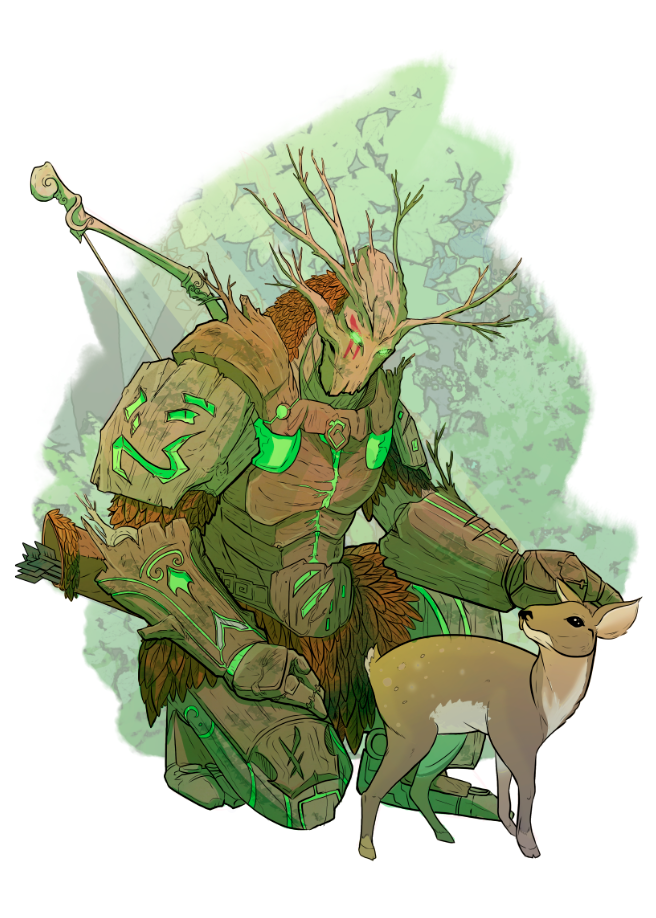
\includegraphics[width=0.48\textwidth]{04kins/img/21quies_druid.png}
% \end{figure}

\subsection*{Traits}
    Designed for efficiency, your quies character has the following traits:

    \subparagraph{Ability Score Increase} Your Constitution and Strength scores increase by 1.

    \subparagraph{Age} Every quies is somewhere between 670 and 890 years old, but their memories before the schism are vague and unreliable.
    Since they've shown no sign of deterioration over time, quies are assumed to be impervious to aging.

    \subparagraph{Alignment} Most quies take comfort in order and discipline, tending toward law and neutrality, but some have chosen a new morality based on the experiences of their independent life.
    They came as a blank slate, and do not tend to any particular tide as a species.

    \subparagraph{Size} Quies are of formidable size, standing between 1.8 and 2.25 meters tall.
    Your build is determined by your subrace.
    Your size is medium.

    \subparagraph{Speed} Your base walking speed is 6 meters.

    \subparagraph{Dual Nature} Due to your manufactured nature, you are both humanoid and construct.
    You can be affected by an effect if it works on either of these two creature types.

    \subparagraph{Quies Resilience} You were created with fortitude in mind.
    You have advantage on saving throws against being poisoned, and you have resistance to poison damage.

    \subparagraph{Integrated Protection} Your body has built-in defensive layers, which can be enhanced with armor:

    \begin{itemize}
        \item You gain a passive +1 to Armor Class.
        \item You can only don armor with which you have proficiency.
        To don armor, you must incorporate it into your body as part of a short rest, during which you remain in contact with the armor.
        To doff armor, you must spend 1 hour removing it.
        \item While you live, your armor can't be removed from your body against your will.
    \end{itemize}

    \subparagraph{Mountain Built} You are impervious to all effects related to altitudes up to 20,000 meters, including cold and lack of oxygen.

\subsubsection{Operative}
    You were designed with a certain specialized function in mind.
    You might be a carpenter, a cartographer, or an entertainer, to name a few possibilities.

    Operatives are the most common of the quies, yet each is of unique design.
    Your build is dependent on the task you were designed for, and you can be as light as 70 kg to as heavy as 150 kg.

    \subparagraph{Ability Score Increase} Any ability score of your choice increases by 1.

    \subparagraph{Integrated Tool} You are competent with one set of artisan's tools or one instrument of your choice.
    This tool or instrument is integrated into your body, and is related to what was your purpose when you lived in Jan'krug.
    You must have your hands free to use this integrated tool.

    \subparagraph{Specialized Design} You are competent with one skill of your choice.

\subsubsection{Juggernaut}
    While many ets were more than capable of dealing with heavy lifting, they designed this branch of quies for fulfilling these tasks in conditions less ideal for them, or simply to work in cooperation with them.
    Juggernauts have a large frame and powerful build, and can weigh up to 230 kg.
    % While these quies were not specifically designed to fight, they usually prove more than capable of melee combat.

    \subparagraph{Ability Score Increase} Your Strength score increases by 1.

    \subparagraph{Hard Fists} Your arms and fists are lined with obsidian, a specially hard stone from the higher parts of the spire.
    When you hit with an unarmed strike, you can deal 1d4 + your Strength modifier bludgeoning damage, instead of the normal damage for an unarmed strike.

    \subparagraph{Powerful Build} You count as one size larger when determining your carrying capacity and the weight you can push, drag, or lift.

% \begin{table*}[b]%
%     \begin{DndTable}[width=\linewidth]{X}
%         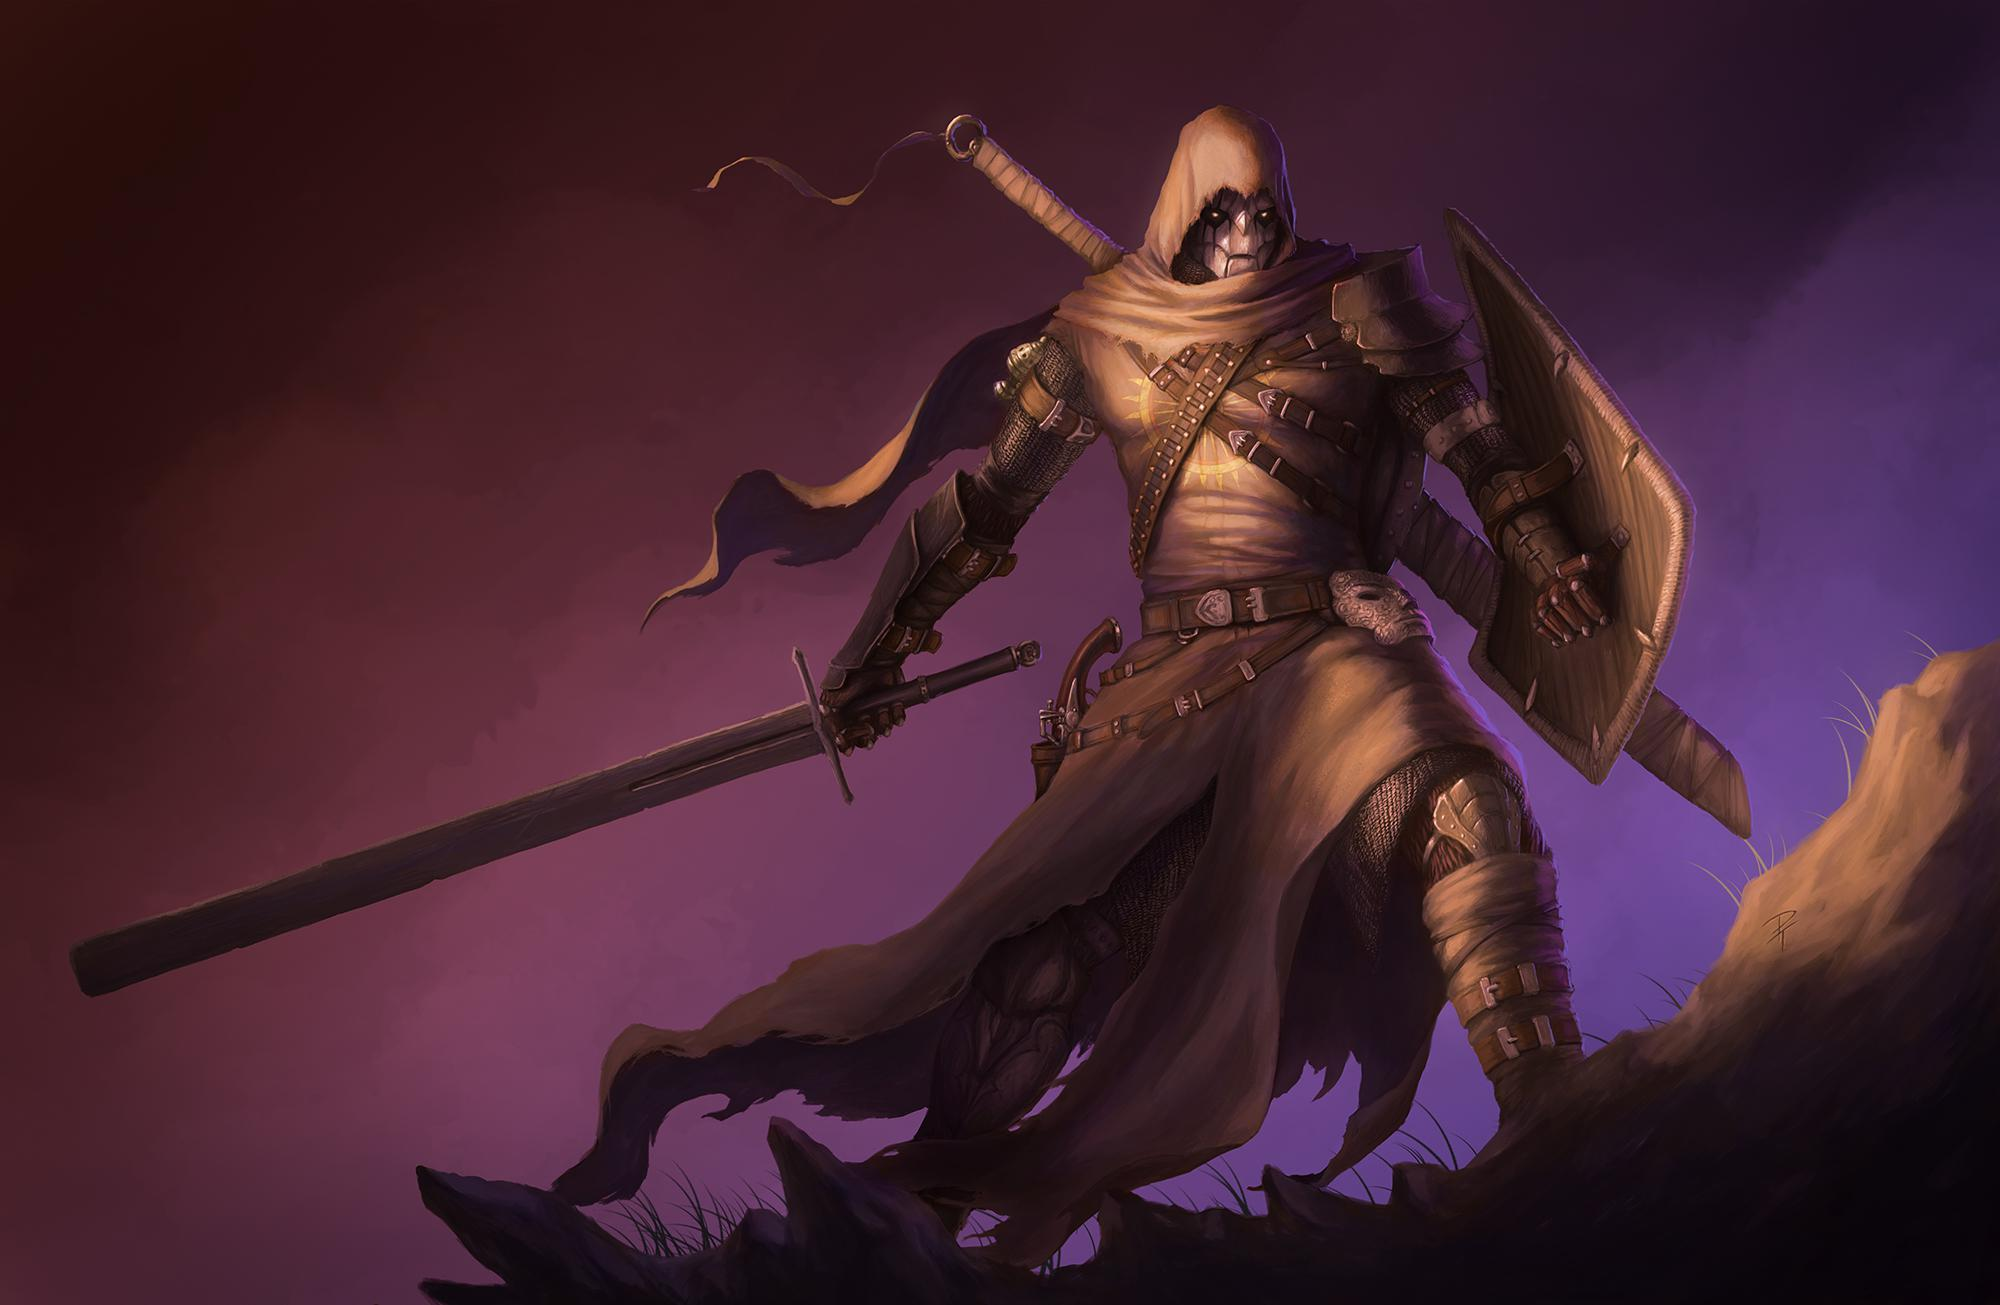
\includegraphics[width=0.98\textwidth]{04kins/img/21quies_executioner.jpg}
%     \end{DndTable}
% \end{table*}

\subsubsection{Slag Worker}
    Even with the adaptable form of the tall kin, not even them can survive the extreme heat of lava for long.
    Consequently, they created the slag workers, quies designed specifically for working inside volcanoes.
    Built to work under extreme pressure, the carapace of the slag workers is a thick layer made from rhyolite.
    While the rock deforms and contorts under lava, it completely blocks the quies from the liquid and its heat.
    % Even the qualar of these quies is infused with the rock, to completely isolate them from their environment.

    \subparagraph{Ability Score Increase} Your Constitution score increases by 1.

    \subparagraph{Heavy Plating} This trait replaces integrated protection.
    You are covered by a rhyolite armor of a light-pink and gray color, containing small vugs filled with obsidian and quartz.
    Your Armor Class is 17, and you have disadvantage of Dexterity (Stealth) checks.
    For all intends and purposes your natural armor is considered Heavy Armor, and it cannot be removed from your body in any way while you are alive.

    \subparagraph{Specialized Worker} You are resistant to fire damage.
    You are also able to enter bodies of lava or magma, sinking at a speed of 5 feet per turn and not suffering any damage while inside.
    For the purposes of moving, lava and magma counts as difficult terrain for you.
    You still need to breathe, and must follow the normal rules for holding your breath while submerged in the hot liquid.

    \subparagraph{Defensive Stance} If you have one hand free, you can choose to enter a defensive stance as an action.
    You add a +3 to your AC until the start of your next turn.
